\chapter{The Survey Results}
\label{chp:surveyresults} 

The survey we created was available for 3 weeks, and in that time period we collected 250 responses from 13 different countries. In this chapter we will go through the results of the survey. First we will go through the demographics to get an image of our respondents. We will then compare and analyze the results with focus on how often the respondents check their Facebook settings, and their app awareness. We looked at how \textit{the ones who have never checked their Facebook privacy settings during the last year}, and \textit{the ones who check their Facebook settings once a month or once a week or more} has changed their settings from the default settings. We then draw some comparisons between these two groups. After this we will look at the questions regarding the users' personal experience. Last, but not least we go through and analyze the questions regarding Facebook apps, and the interdependent privacy issues related to them.
From these analysis we investigate the following hypothesis: \textit{"The ones with many apps have less knowledge about the privacy issues related to apps."}

\section{Demographics}

\begin{figure}[h!]
\centering
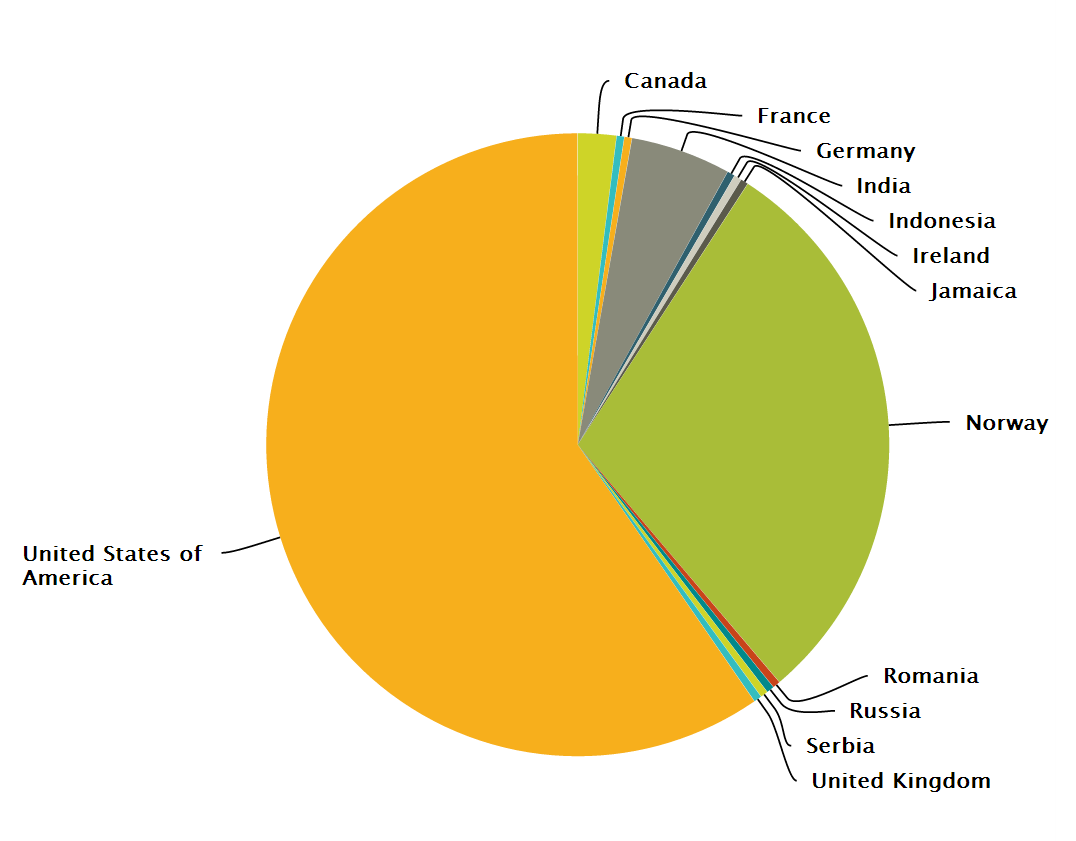
\includegraphics[width=1\textwidth]{land.png}
\caption[Total distribution of the participant's country of origin]{\textbf{Total distribution of the participant's country of origin.} Most of the participants are from the United Stated of America and Norway.} 
\label{fig:land}
\end{figure}


As mentioned before, we distributed our survey on two platforms; Amazon Mechanical Turk (AMT) and Facebook. In total, we received 250 responses from 13 different countries. As you can see in \fref{fig:land}, the distribution of countries was mainly divided between two, the United States of America and Norway. Other countries were also represented; Canada, France, Germany, India, Indonesia, Ireland, Jamaica, Romania, Russia, Serbia and United Kingdom. 77 of the 250 responses were collected through the Facebook link, and out of these people 96\% (74 people) were from Norway. 173 of the 250 respondents took the survey via Amazon Mechanical Turk, and out of these people 85.5\% (148 people) were from the United Stated of America. 

\paragraph{Gender.}

\begin{figure}[h!]
\centering
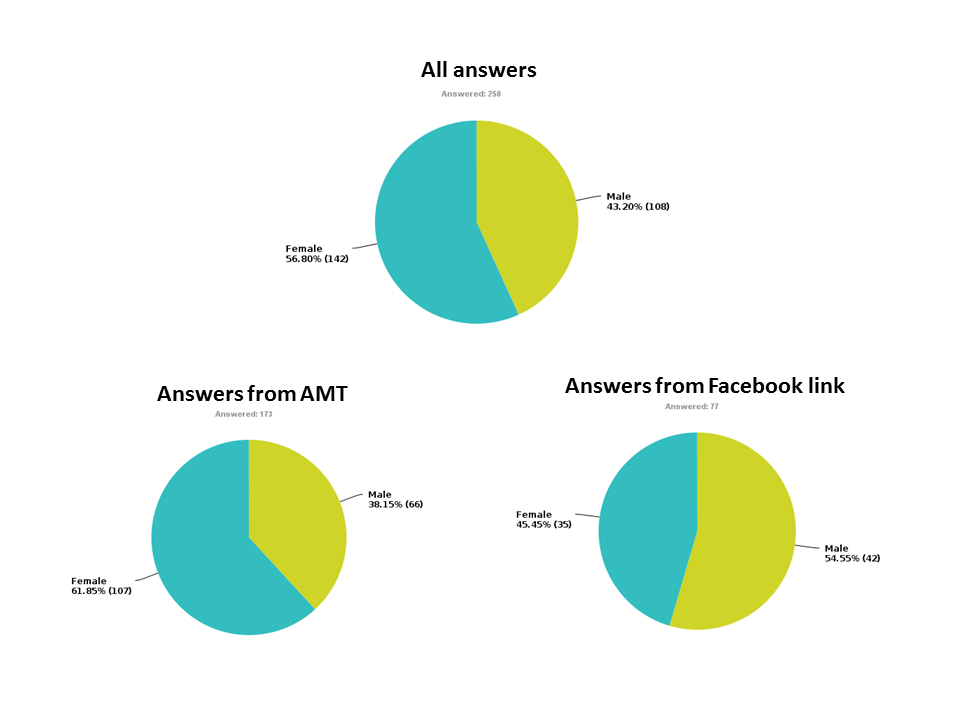
\includegraphics[width=1\textwidth]{gender.png}
\caption[Gender distribution]{\textbf{Gender distribution}. This graph shows the overall gender distribution (on the top), gender distribution from AMT (to the left) and the gender distribution from the Facebook link (to the right).} 
\label{fig:gender}
\end{figure}

The majority of the total respondents were female. They accounted for 56.80\% of the responses (142). This means that 43.20\% of the total respondents were male, with a 108 responses. We saw a difference in the gender distribution from the Facebook link and from AMT. On AMT 38.15\% were men, and 61.85\% were female. On Facebook 54.55\% were male, and 45.45\% were female. In other words the majority of respondents on AMT were females, in contrary to Facebook, were the majority of respondents were men. The difference in gender distribution is shown in the \fref{fig:gender}.

\paragraph{}
Among the participants, the age ranged between 19 and 76. The average age was 31. If we look at the difference in age between the respondents from AMT and Facebook, we see that the average age of the AMT respondents is 33 and the average age of the Facebook respondents is 27. In others words the AMT respondents have a higher average age than the respondents from Facebook. 

%DISCUSSION: This difference in age comes from the fact that most of the respondents from Facebook were our friends, and most of them are in their mid-twenties. 

When we look at the total income of the household per year and employment status, we found a wide range of variety among the participants. We had several participants in each group of income. Although the majority of the participants were employed for wages or students, all of the other employment statuses was represented. This was consistent with former studies of AMT users \cite{incentivesAmt}. 


\section{Never Checked Facebook Privacy/Security Settings During the Last Year}

30 of the people who answered our survey stated that they have never checked their settings during the last year. Even though they have not checked their  settings during the last year, most of them have done some changes to their settings before the previous year. The reason for this assumption is that their settings differ from the default settings.  
The average number of friends for the people who have never checked their Facebook settings during the last year is 162, and their average age is 39. 

\begin{figure}[h!]
\centering
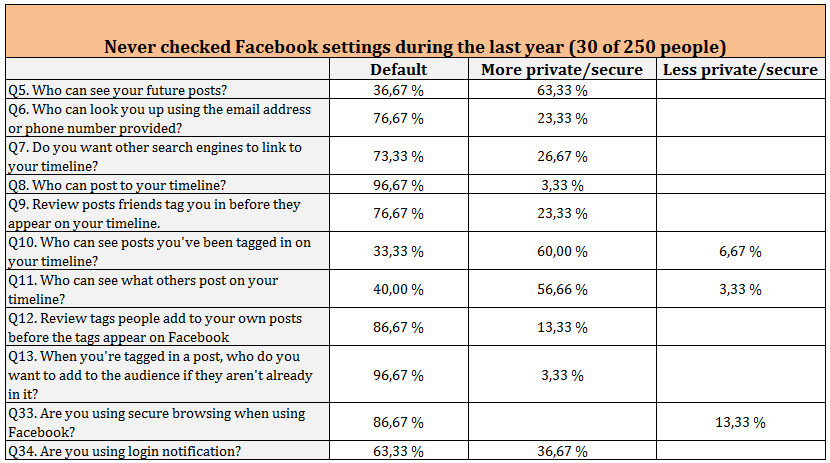
\includegraphics[width=1\textwidth]{nevercheckedtable.png}
\caption[Never checked Facebook privacy/security settings during the last year]{\textbf{Never checked Facebook privacy/security settings during the last year.}} 
\label{fig:neverchecked}
\end{figure}

In \fref{fig:neverchecked} you can see the percentage distribution over Facebook settings among the people who have never checked their Facebook privacy settings during the last year. We have divided these respondents into tree categories; "Default", "More private/secure", and "Less private/secure". The respondents end up under the category "Default" if their setting is similar to the default setting anno 2013. See section \ref{subsec:default2013} for more detailed description of the default settings on Facebook. The respondents end up under the "More private/secure" category if their settings have been changed from the default setting to a more secure setting. The "Less private/secure" is for those who have made changes to their setting which is less secure than the default setting. As shown in \fref{fig:neverchecked}, the majority of these respondents have not changed their settings from the default settings. 

The majority of these users are active users, 67\% of them checks their Facebook page at least once a day. 60\% of the people who had never checked their Facebook settings during the last year \textit{did not} consider changing their settings after reviewing them. 40\% of them wanted to make their settings more private/secure. 

%DISCUSSION:

\begin{quote}
\textit{"Now you have scared me. I am alone and afraid."} - 67 year old woman with Ph.D and 5 Facebook friends. 
\end{quote}

\subsection{App awareness}
73.33\% of these 30 respondents were aware of the fact that all apps on Facebook access their basic information. Less of them were aware that many apps post on your behalf (56.6\%). \fref{fig:appawarenessneverchecked} shows the percentage distribution from the questions regarding apps' permission requests (Questions 25-29 in \fref{fig:page14} and \fref{fig:page15}). The two on top shows the ones just mentioned respectively. As you can see, the amount who answered "No" increased drastically on the last two questions. The third question asks for the users awareness regarding the fact that some apps access your friends' private information, and the fourth and last regard the fact that some apps have access to relational information (such as private chat messages). 

\begin{figure}[h!]
\centering
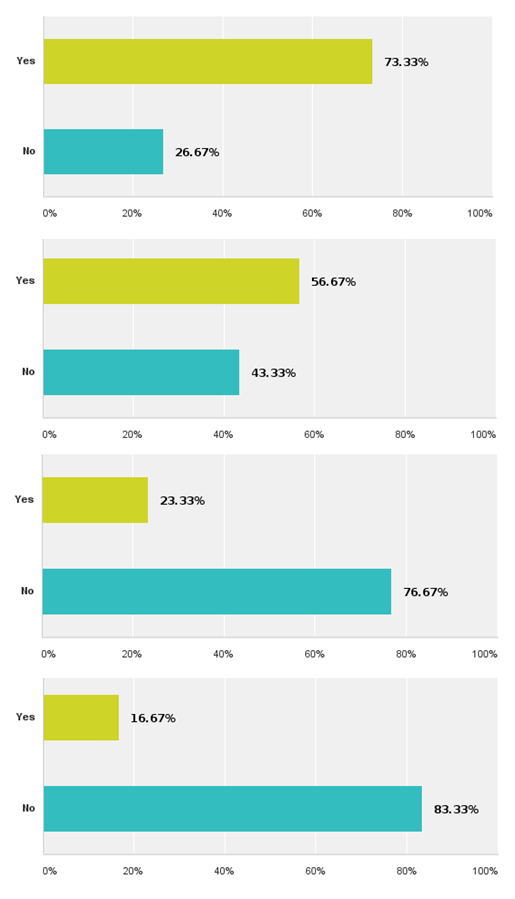
\includegraphics[width=0.6\textwidth]{q26-29AppAwareness.png}
\caption[The distribution of question 26-29, showing app awareness among the 30 respondents that have never checked their Facebook settings during the last year]{\textbf{The distribution of question 26-29, showing app awareness among the 30 respondents that have never checked their Facebook settings during the last year.}} 
\label{fig:appawarenessneverchecked}
\end{figure}


\section{Checks Facebook Privacy/Security Settings "Once a month" or "Once a week or more"}

\begin{figure}[h!]
\centering
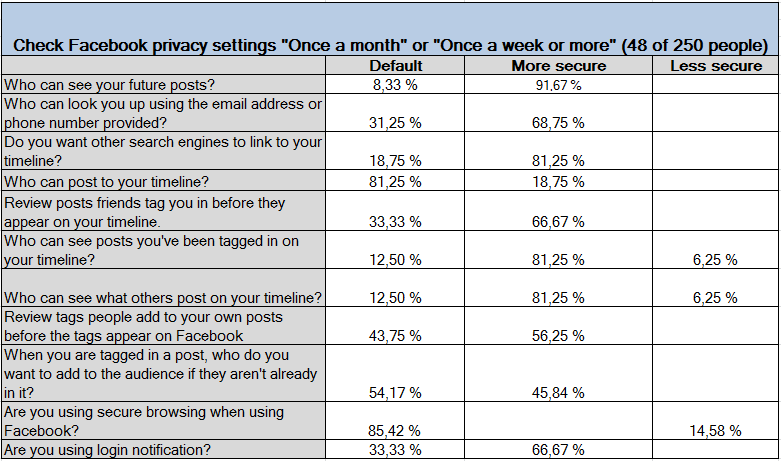
\includegraphics[width=1\textwidth]{checkonceaweekormoretable.png}
\caption[Checks Facebook privacy/security settings "Once a month" or "Once a week or more"]{\textbf{Checks Facebook privacy/security settings "Once a month" or "Once a week or more".}} 
\label{fig:onceaweekormore}
\end{figure}

48 of the people who answered our survey stated that they check their settings "Once a month" or "Once a week or more". The average number of friends for these people is 416, and their average age is 28.5. The average age of this group is almost 10 years lower than for the group of people that have not checked their settings during the last year.

In \fref{fig:onceaweekormore} you can see the percentage distribution of what kind of settings the people who check their settings "Once a month" or "Once a week or more" have. We have divided them into the same categories as above; "Default", "More private/secure", and "Less private/secure".  

85\% of the people who checked their Facebook settings "Once a month" or "Once a week or more" during the last year, has checked their Facebook page at least once a day during the last month. This indicates that the majority of those who check their settings frequently are also very active Facebook users. 

70.83\% of these people did not consider changing their settings after reviewing them. 27.08 \% wanted to make their settings more private/secure, and 2.08\% considered changing them to more public. 


%12 of the 48 people in this category answered yes on the question whether or not facebook had affected their personal life negativally. Half of these had situations with friends posting unwanted pictures (av forskjellige grunner) of them.

\begin{quote}
\textit{"Privacy is important to me. It is meaningless not to give others the same courtesy"} - 43 year old man with 420 Facebook friends. 
\end{quote}


\subsection{App awareness}
72.92\% of these 48 respondents were aware of the fact that all apps on Facebook access their basic information. A larger number of these respondents were aware that many apps post on your behalf (81.25\%). \fref{fig:appawarenessonceaweek} shows the percentage distribution from four of the app awareness questions (Questions 25-29 in \fref{fig:page14} and \fref{fig:page15}). The two on top shows the ones just mentioned respectively. As you can see, the share who answered "No" increased on the last two questions. The third question asks for the users awareness regarding the fact that some apps access your friends' private information, and the fourth and last regard the fact that some apps have access to relational information (such as private chat messages).  

\begin{figure}[h!]
\centering
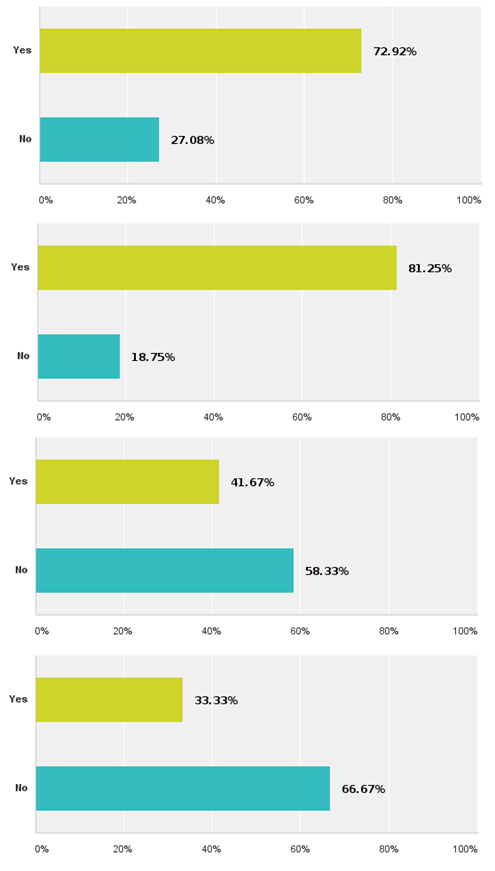
\includegraphics[width=0.6\textwidth]{q26-29OnceAWeek.png}
\caption[The distribution of question 26-29 showing app awareness among the 48 respondents that checks their Facebook settings "Once a month" or "Once a week or more"]{\textbf{The distribution of question 26-29 showing app awareness among the 48 respondents that checks their Facebook settings "Once a month" or "Once a week or more".}} 
\label{fig:appawarenessonceaweek}
\end{figure}


\section{Comparing the ones who never check and the ones who check frequently} 

\subsection{Activity level}
The majority of both groups checks their Facebook page at least once a day. The percentage is higher for the people who have checked their settings "Once a month" or "Once a week or more" during the last year. 85\% of them checks their Facebook page at least once a day, in contrast to the other group (who have never checked their settings during the last year) with 67\% checking their Facebook page at least once a day. This indicates that the ones who have never checked their settings during the last year does not refrain from doing this because they are inactive users. One assumption for this may be that the users are unaware of the settings. 40\% of them stated that they wanted to make their settings more private after taking the survey. This backs up the assumption about unawareness.  


\subsection{More secure settings for those who check their settings more often?}
If we compare \fref{fig:neverchecked} and \fref{fig:onceaweekormore}, we see a clear difference in percentage that have changed from default to a more secure option. The percentage of changes to a more private/secure option is much higher for all settings listed for those who checks frequently. Some of the settings shows a remarkable difference between the groups. We want to accentuate the settings that concern interdependent privacy. When we look at the setting "Review posts friends tag you in before they appear on your timeline" for the ones that never checked during the last year, only 23.33\% have changed to a more secure option. For the ones that check frequently, 66.67\% have changed to a more secure option. Another example is the setting "Review tags people add to you own posts before the tags appear on Facebook" where 13.33\% of the ones who never have checked their settings during the last year changed to a more secure option. On the contrary, as many as 56.25\% of the frequent settings-checkers have changed to a more secure option.

\subsection{Considered changing settings}
The percentage of those wanting to make their settings more private is higher for those who have never checked settings during the last year with 40\% of the group. Only 27\% of the frequent setting-checkers wanted to make their settings more private. 
None of the people who have never checked their settings during the last year wanted to make their settings more public, unlike the other group (those who check "Once a month" or "Once a week or more") where 2\% actually considered changing them to more public. Overall the frequent settings-checkers were more pleased with their settings than the once who had never checked them during the last year. 70\% of the frequent settings-checkers did not consider changing their settings after reviewing them. Although the ones who have never checked their settings during the last year have far less secure settings than the other group, 60\% of them did not consider changing their settings either. 

\section{Comparisons with Previous Surveys} 
In the article "Analyzing Facebook Privacy Settings: User Expectations vs. Reality" \cite{expectations} they found that modified privacy settings match the users expectations only 39\% of the time (This is elaborated in section \ref{sec:relatedwork_facebookprivacy}). In our case this number is much higher, 65.6\% stated what they did not consider changing their privacy settings after reviewing them. This is an interesting observation. The previous research was done in 2011, and a lot has changed since then with regard to privacy settings. One assumption is the ongoing attention towards online security. With the media trying to make people aware of how easy it is to access ones information on the web. 

In the other article mentioned in \ref{sec:relatedwork_facebookprivacy}, "Facebook privacy settings; Who cares?" \cite{whocares} they found that among the majority both genders were equally confident in changing their Facebook privacy settings. Our survey backs up this finding to some extent. The majority of both females and males have changed their settings to a more private option, but our research shows that females focus more on who can see their posts and posts they have been tagged in and who can look them up. 83.1\% of the females have changed the settings "Who can see posts you've been tagged in on your timeline?" to a more private option and 80,25\% of the females have changed the setting "Who can see what other's post on your timeline?" to a more private option. In both of these settings, this is almost 10\% more than for males. In contrary, males have a larger focus on security, with more secure options on settings like "Login notification" and "Secure browsing". 

\section{Users' personal experience}
Out of the 250 respondents 11 answered yes on the question "Have you ever experienced that your use of Facebook has affected your professional life?". 3 of these 11 have had their professional life affected in a negative way, and 8 was affected in a positive way. 

50 of the 250 respondents stated that their use of Facebook had lead to uncomfortable situations, for example concerning unpleasant messages and/or inappropriate comments or pictures. The majority of the situations concerns unwanted pictures (where they do not look good) shared beyond their preferred audience and inappropriate comments on pictures of them. Some also mention cases of stalking. Some of the comments are shown below:

\begin{itemize} 
\item "\textit{I had a friend I parted ways with harass me on Facebook by threatening messages, posts to photos about me, etc. I also had sexual harassment over Facebook message by an ex boyfriend, inappropriate comments and propositions I was not interested in.}"
\item "\textit{Before I changed my settings, someone posted a picture of me that I did not want to share with everyone else.}"
\item "\textit{An ex girlfriend was using Facebook to get information about me and my friends.}"
\item "\textit{I shared (public) a photo from a friends timeline which he had posted to a limited set of friends, he got mad.}"
\item "\textit{I have many younger friends on Facebook (underage), and I would like to be a good role model. So sometimes there have been pictures of me consuming alcohol, and I don´t want my younger friends to see that. I now have customized my settings, so they only see my personal posts which dosen´t include alcohol/smoking etc.}"
\item "\textit{Someone commented something on a photo I was tagged in that I don't want everyone to know about me}"
\item "\textit{I girl posted a naked photo of me.}"
\item "\textit{Just pictures of me not looking my best being posted by friends who then tag me and suddenly everyone - friends of friends, etc. can see the pics. It wasn't disasterous or inappropriate, but those weren't pictures I wanted old classmates from high school to look at (unless we are friended on FB)}"
\end{itemize}

39.6\% of the total respondents have blocked one or more due to uncomfortable situations or harassment. 

To see how much a person values their privacy, we asked them to state on a scale from 1 to 5 to what degree they care about what is published about themselves. 1 is "I don't care at all. Everything can be public" and 5 is "I untag and hide everything that is published of me". The majority (35.6\%) answered 3 on the scale.  When people were asked to elaborate on this topic, the comments ranged from \textit{"I don't trust the Internet"} to \textit{"I don't untag everything, because the point of the site is to be social"}. Many says that they frequently untag photos they do not want others to see. One of the respondents said \textit{"It's a tricky dilemma, because when you untag you also loose control over what happens with the picture/post"}.

From our results, it seem like people care more about what they post of others, than what is posted about themselves. When we asked them to what degree they are selective about what they post about others on a scale from 1 to 5, where 1 is "I am not selective at all, I post everything" and 5 is "I never post anything about anyone", the majority answered 4. This shows that people are very selective when it comes to posting things about others. When people were asked to elaborate on this topic, the comments ranged from \textit{"I post whatever I want without care"} to \textit{"I think before posting how what I am posting might affect myself and the person I am tagging or may be in the picture. I understand that some content can have affects on others"}.

\section{Interdependent Privacy}

A big part of our survey focus on apps and the issues related to apps which concerns interdependent privacy. When installing an app on Facebook, most apps ask for permission to access information in addition to your basic information (name, profile picture, cover photo, gender, networks, username, user ID, your list of friends, and any information you choose to make public). We wanted to map the awareness of the respondents when it came to apps, and to what degree they knew about the information apps access. 

\subsection{Users' knowledge about the term "Interdependent Privacy"}
We also wanted to find out whether or not the respondents had knowledge about the term interdependent privacy. We asked the question "Do you have any idea about what interdependent privacy can mean in regard to Facebook?" both before and after the app-related questions. We specified in the question that they were not allowed to use Google or any other search engine to find the answer. If they did not know the answer it would be preferable for us if they skipped the question. It would not be of any value for us, if they searched for the "definition". We wanted to see if people could come up with their own idea of the term. 136 of the 250 respondents answered that they did not know the meaning of the term, or skipped the question, both before and after the app-related questions. 69 of the respondents skipped the first time they were asked about the term, but answered the second time. Even though everything was not entirely correct, a lot of people seemed to have gotten some idea of what the term evolves around after answering the question about apps. \tref{tab:thoughtonintpriv} shows some of the answers, both before and after the app-related questions. See Appendix \ref{chp:appendixB} for all responses.   


\begin{center}
\begin{longtable}{ | p{6cm} | p{6cm} |}
    \caption{\label{tab:thoughtonintpriv}Peoples thoughts of what is meant by interdependent privacy before and after answering questions about privacy issues regarding the use of Facebook apps.} \\
    \hline
\textbf{Q24. Do you have any idea about what interdependent privacy means?} & \textbf{Q31. Do you have any idea about what interdependet privacy means after answering questions regarding privacy issues using Facebook apps?} \\ 
\hline
\textit{"I have no idea what interdependent privacy means. It almost does not make sense to put those two words together. If you have privacy, it should not depend on another party to make it private. That defetes the whole purpose of "private"."} &  \textit{"Hmn. I guess it makes sense now, seeing that apps can do that to people who are friends."}\\ 
    \hline
\textit{"I would image it relates to one person's privacy being compromised or supported by another user's privacy settings."} & \textit{"Yes, I understand what it means now. If a friend of mine permits an app to access their info then they have a certain amount of access to my info."}\\ 
    \hline
\textit{"I think it's when my picture is visible to only friends but then a friend of mine reshares it, so I have to rely on that friend to keep my stuff private too."} &  \textit{"I think I was close to right. Relying on others' settings to keep my privacy."}\\ 
    \hline
\textit{"I think it means that people you allow to see things can also allow others to see it if they chose to, with or without your permission but I am not sure about this."} & \textit{"I think that it means if you give an app permission to use your information, the app can then use the information in any way it wants to. This is why I do not use any apps because I do not trust them period."}\\
    \hline
\textit{"I think it has to do with other sites and apps allowing you to sign into or register for accounts using your facebook account.  You would now have another set of privacy policies to review and how the two sites work together"} & \textit{"Apps you use can disregard your privacy settings with facebook and play by tehir own rules - so I have to be much more diligent."}\\
	\hline
\textit{"I think it means that people you allow to see things can also allow others to see it if they chose to, with or without your permission but I am not sure about this."} & \textit{"I think that it means if you give an app permission to use your information, the app can then use the information in any way it wants to. This is why I do not use any apps because I do not trust them period."}\\
    \hline
\textit{"It's something about where someone else saying something (like Bob saying "Bob is at the restaurant with Mike") can reveal information about another person (in this case, that Mike is at the restaurant)."} & \textit{"Maybe it's: Facebook taking other people's info based on something I do."} \\
    \hline
   \textit{ "My privacy can be affected by those I share with. Just because I make something private does not mean that my friends won't pass it along, making it no longer private."} & \textit{"You are not the only person in control of your privacy. If you don't use the right settings, other people can share information you think is private."}\\ 
    \hline  
\textit{"I have no control over what info my friends share about me"} & (Skipped) \\
    \hline
\textit{"Nope. I will for sure google it now."} & \textit{"That it´s obv. not only facebook who can access my privacy settings, that this so called privacy is interdependet and I am in charge of setting those settings myself if I don´t want it to be that interdependent."} \\
    \hline
\textit{"What others can do to your privacy if you "let them"?"} & \textit{"Yes. what concerns your privacy that you dont know of, that your friends do to your privacy ish."}\\ 
    \hline  
\textit{"My privacy depends on others"} & \textit{"The apps are allowing people to see things that are private. It's interdependent on FB."}\\ 
    \hline
\textit{"I would say it means it depends on what others would post or say about you, or give out your private things."} & \textit{"You can control what you share, but not what others do or say that may infringe on your privacy."}\\ 
    \hline 
\textit{"No"} & \textit{"Getting access through games and friends."} \\ 
    \hline
(Skipped) & \textit{"My privacy setting depends also on other users, with the help of apps. I think this is what interdependent privacy means."}\\ 
    \hline
(Skipped) & \textit{"Maybe other apps can take information from your friends without their knowing."}\\ 
    \hline    
(Skipped) & \textit{"It seems to be privacy independent from privacy settings. It appears apps can override general privacy settings."}\\ 
     \hline
(Skipped) & \textit{"That apps I put on my FB page can access my friend's accounts, information and activities. I am always very careful to select "ONLY ME" when they ask whose wall they can post to - but I wasn't aware that apps were independently able to access the information of my friends without my consent."}\\ 
     \hline 
(Skipped) & \textit{"I think that it means that the apps that I use can have an effect on my friends privacy."}\\ 
     \hline     
    \end{longtable}
\end{center}

An issue discussed in the paper "Third-Party Apps on Facebook: Privacy and the Illusion of Control" \cite{thirdPartyApps} is the importance of user control of apps' data access, and that it should be made clear to the user what information they give the apps permission to access. In this paper, they conclude that it is often unclear to the users what information they agree to share, and that apps often ask for permissions that are in conflict with their privacy settings. We wanted to see if the users were aware of what information apps may ask for, and how much information they may agree on sharing (not just about themselves). 

\subsection{Number of apps connected to Facebook}
In the apps settings, one can see a list of all the apps the user have connected to Facebook. \fref{fig:appsyouuse} show the amount of apps the respondents have. The distribution is close to even for all the alternatives. 86.8\% of the total respondents have at least one app connected to their Facebook. A higher percentage of the respondents have more than 30 apps connected to their Facebook, than none apps. 

\begin{figure}[h!]
\centering
\fbox{
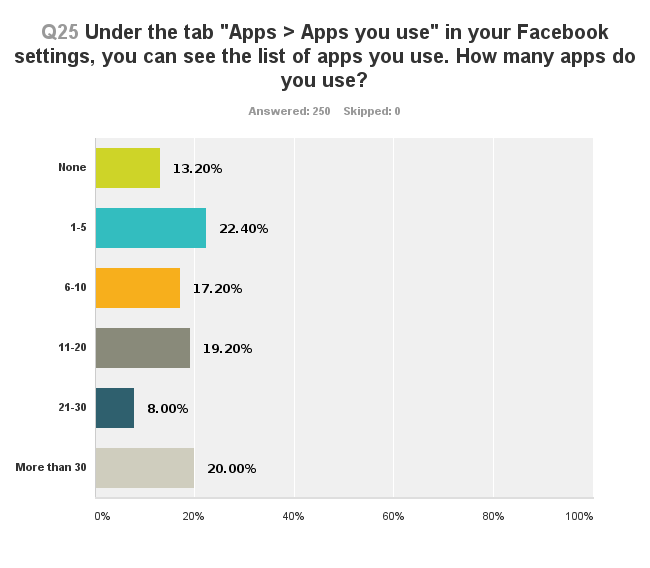
\includegraphics[width=0.8\textwidth]{appsyouuse.png}}
\caption[Question 25 - Displaying the distribution of number of apps among the 250 respondents]{\textbf{Question 25 - Displaying the distribution of number of apps among the 250 respondents.}} 
\label{fig:appsyouuse}
\end{figure}

\subsection{Users' awareness regarding app permission requests}
\fref{fig:appsaccessbasicinfo}, \fref{fig:appspostonyourbehalf}, \fref{fig:appsaccesstofriendsinfo} and \fref{fig:appsaccessrelationalinfo} show the results from question 26, 27, 28 and 29, where we ask the respondents about their awareness regarding the information apps request. The two first figures (concerning basic information and apps posting on your behalf) shows that the majority of the respondents were aware of the facts presented. The two last figures, on the other hand, show that the majority were unaware of the permission requests. The two first questions are more visible for the users, it is stated many times that all apps access your basic and public information, and the users experience apps posting both on their behalf and on friends' behalf (for example Spotify posting play lists or songs you have listened to). The two last questions (concerning friends private information and access to relational information)are more hidden from the users, because nothing is posted or viewable etc. The users are not notified when the apps access this information, and therefore have no idea of what is specifically retrieved, when it is used, and for what purpose. We therefore think it is less knowledge about these permission requests. 

\begin{figure}[h!]
\centering
\fbox{
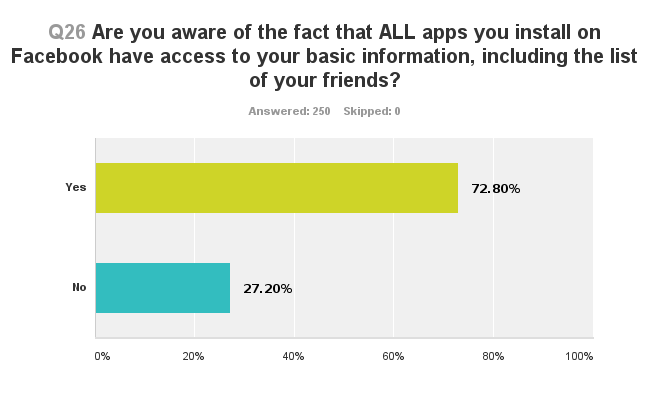
\includegraphics[width=0.8\textwidth]{appsaccessbasicinfo.png}}
\caption[Question 26 - Displaying the awareness of the fact that all apps access your basic information]{\textbf{Question 26 - Displaying the awareness of the fact that all apps access your basic information.}} 
\label{fig:appsaccessbasicinfo}
\end{figure}

\begin{figure}[h!]
\centering
\fbox{
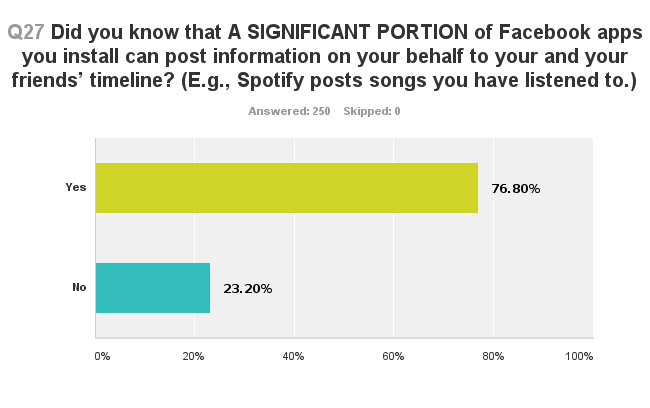
\includegraphics[width=0.8\textwidth]{appspostonyourbehalf.png}}
\caption[Question 27 - Displaying the awareness of the fact that a significant portion of apps post on your behalf]{\textbf{Question 27 - Displaying the awareness of the fact that a significant portion of apps post on your behalf.}} 
\label{fig:appspostonyourbehalf}
\end{figure}

\begin{figure}[h!]
\centering
\fbox{
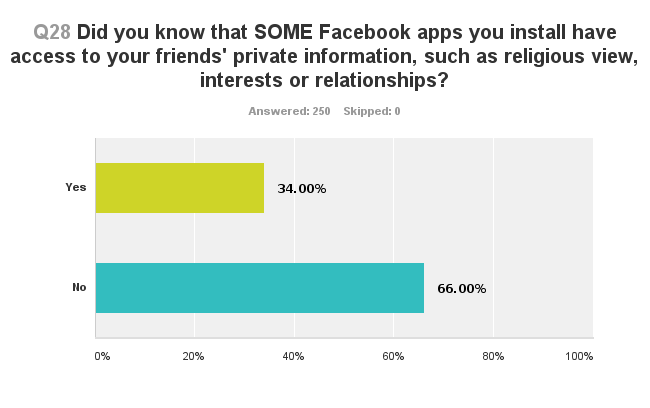
\includegraphics[width=0.8\textwidth]{appsaccesstofriendsinfo.png}}
\caption[Question 28 - Displaying the awareness of the fact that some apps access your friends' private information]{\textbf{Question 28 - Displaying the awareness of the fact that some apps access your friends' private information.}} 
\label{fig:appsaccesstofriendsinfo}
\end{figure}

\begin{figure}[h!]
\centering
\fbox{
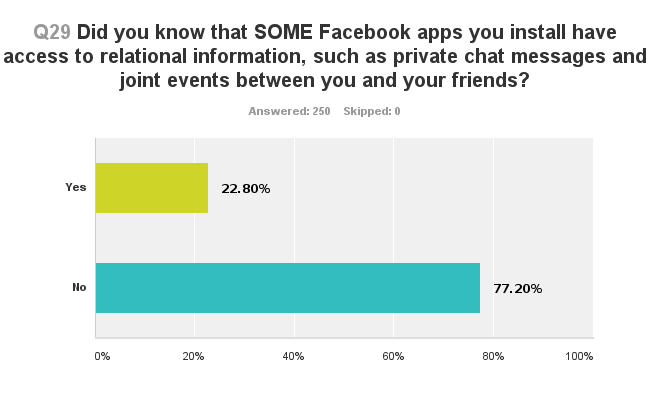
\includegraphics[width=0.8\textwidth]{appsaccessrelationalinfo.png}}
\caption[Question 29 - Displaying the awareness of the fact that some apps access relational information]{\textbf{Question 29 - Displaying the awareness of the fact that some apps access relational information.}} 
\label{fig:appsaccessrelationalinfo}
\end{figure}



\subsection{Hypothesis: the ones with many apps have less knowledge about the privacy issues related to apps}

\begin{figure}[b]
\centering
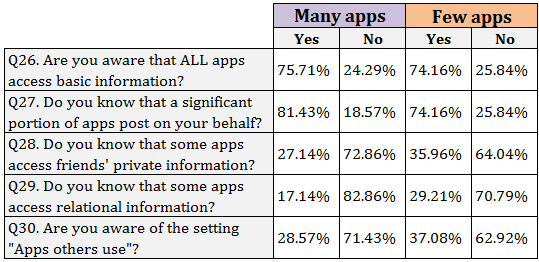
\includegraphics[width=0.8\textwidth]{awareness(manyappsandfewapps).png}
\caption[App awareness - Comparing those with many app and those with few apps]{\textbf{App awareness - Comparing those with many app and those with few apps.} Percentage distribution of the answers to all of the app questions differentiating the 70 people with many apps (21 apps or more) and the 89 people with few apps (5 or less).} 
\label{fig:manyappsandfewapps}
\end{figure}

We wanted to find out whether or not people using many apps had more or less knowledge when it came to the app-related questions, than people using few apps. Our hypothesis were that the ones with many apps have less knowledge about the privacy issues related to apps. The reason for this assumption is that we thought if people were aware of all the permissions they agree/agreed on, they would not have had that many apps to begin with, because of the privacy breach apps cause. In other words, we thought that those with few apps had more knowledge about the privacy issues related to apps, and therefore chose to refrain for installing apps and/or are frequently deleting the apps not in use.
\fref{fig:manyappsandfewapps} shows the results of this comparison. On question 26 the distribution is close to equal for those with many apps (21 apps or more) and those with few (5 apps or less). This is a relatively common known fact, because information about this is stated on the top of the app settings, as well as always on top of the list when installing an app. Question 27 shows that the people with many apps were more aware of the fact that a significant portion of apps post on your behalf. We think the reason for this is that the people who frequently use apps have more experience when it comes to apps posting on their behalf, and this makes them more aware of this fact. When apps post on behalf of a user, it is shown as a post on their timeline. This is something the user experiences hands on. In addition to this, people who use many apps sees the permission requests from Facebook more frequently. Question 28 and question 29 on the other hand, are not visible for the naked eye. Although, this is stated in the permission request, it is never visible for the user what information is accessed and retrieved by the apps. The percentage of people aware of the facts presented in question 28 and question 29, is higher for those with few apps than for those with many apps. This backs up our hypothesis. The last question (30) concerns the setting "Apps others use" found under the App tab in your Facebook settings. Here the user can choose which information the apps your friends install can access. From our results you see that 37.08\% of those with few apps were aware of the existence of this setting. Almost 10\% less of the ones with many apps were aware of it. This also backs up our hypothesis that the ones with few apps are to a larger extent aware of the privacy issues related to apps and the settings that exist. 

\begin{figure}[t]
\centering
\fbox{
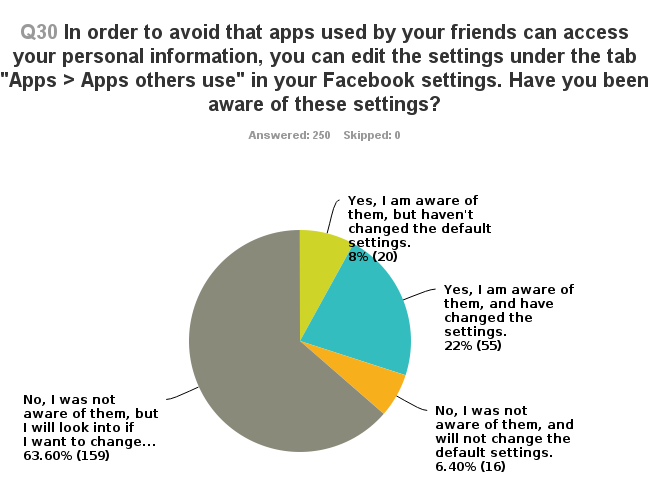
\includegraphics[width=0.8\textwidth]{appsothersuse.png}}
\caption[Question 30 - Displaying the awareness of the setting "Apps others use" among all of the 250 respondents]{\textbf{Question 30 - Displaying the awareness of the setting "Apps others use" among all of the 250 respondents.}} 
\label{fig:appsothersuse}
\end{figure}

\subsection{Awareness of the setting "Apps others use"}
\paragraph{}
Question 30 (\fref{fig:appsothersuse}) does not only ask for a simple "Yes" or "No" answer to whether or not they are aware of the setting "Apps others use". The possible answers for the question is "Yes, I am aware of them, but I haven't changed the default settings", "Yes, I am aware of them, and have changed the settings", "No, I was not aware of them, and will not change the default settings" and "No, I was not aware of them, but will look into if I want to change my settings now". The latter option was significantly higher for those with many apps (see \fref{fig:appsothersusemanyfew}), which means a higher portion of those with many apps were unaware of this setting and dissatisfied with the configuration of their setting, compared to the ones with few apps. Another observation is that the alternative "Yes, I was aware of them, and have changed the settings" is higher for those with few apps. The results shown in \fref{fig:appsothersusemanyfew} backs up our hypothesis that the ones with many apps have less knowledge about the privacy issues related to apps.

\begin{figure}[h!]
\centering
\fbox{
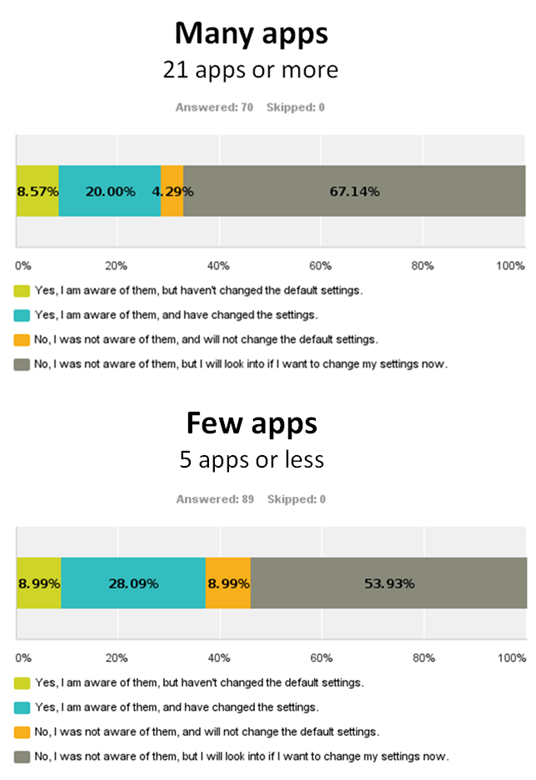
\includegraphics[width=0.7\textwidth]{appsothersusemanyfew2.png}}
\caption[Awareness of the setting "Apps others use" - Comparing those with many app and those with few apps]{\textbf{Awareness of the setting "Apps others use" - Comparing those with many app and those with few apps.}} 
\label{fig:appsothersusemanyfew}
\end{figure}
